\documentclass[
  captions=tableheading,
  bibliography=totoc, 
  titepage=firstiscover,
]{scrartcl}

\usepackage{blindtext} %neuer input

\usepackage{longtable} % Tabellen über mehrere Seiten

\usepackage[utf8]{inputenc} %neuer input

\usepackage{scrhack}

\usepackage[aux]{rerunfilecheck} %Warnung falls nochmal kompiliert werden muss

\usepackage{fontspec} %Fonteinstellungen

\recalctypearea{}

\usepackage[main=ngerman]{babel} %deutsche Spracheinstellung

\usepackage{ragged2e} %neuer input

\usepackage{amsmath, nccmath}

\usepackage{amssymb} %viele mathe Symbole

\usepackage{mathtools} %Erweiterungen für amsmath


\DeclarePairedDelimiter{\abs}{\lvert}{\rvert}
\DeclarePairedDelimiter{\norm}{\lVert}{\rVert}

\DeclarePairedDelimiter{\bra}{\langle}{\rvert}
\DeclarePairedDelimiter{\ket}{\lvert}{\rangle}

\DeclarePairedDelimiterX{\braket}[2]{\langle}{\rangle}{
#1 \delimsize| #2
}

\NewDocumentCommand \dif {m}
{
\mathinner{\symup{d} #1}
}


\usepackage[
  math-style=ISO,
  bold-style=ISO,
  sans-style=italic,
  nabla=upright,
  partial=upright,
  warnings-off={
    mathtools-colon,
    mathtools-overbracket,
  },
]{unicode-math}

\setmathfont{Latin Modern Math}
\setmathfont{XITS Math}[range={scr, bfscr}]
\setmathfont{XITS Math}[range={cal, bfcal}, StylisticSet=1]


\usepackage[
  locale=DE,
  separate-uncertainty=true,
  per-mode=reciprocal,
  output-decimal-marker={,},
]{siunitx}

\usepackage[autostyle]{csquotes} %richtige Anführungszeichen

\usepackage{xfrac}

\usepackage{float}

\floatplacement{figure}{htbp}

\floatplacement{table}{htbp}

\usepackage[ %floats innerhalb einer section halten
  section,   %floats innerhalb er section halten
  below,     %unterhalb der Section aber auf der selben Seite ist ok
]{placeins}

\usepackage[
  labelfont=bf,
  font=small,
  width=0.9\textwidth,
]{caption}

\usepackage{subcaption} %subfigure, subtable, subref

\usepackage{graphicx}

\usepackage{grffile}

\usepackage{booktabs}

\usepackage{microtype} %Verbesserungen am Schriftbild

\usepackage[
backend=biber,
]{biblatex}

\addbibresource{../lit.bib}

\usepackage[ %Hyperlinks im Dokument
  german,
  unicode,
  pdfusetitle,
  pdfcreator={},
  pdfproducer={},
]{hyperref}

\usepackage{bookmark}

\usepackage[shortcuts]{extdash}

%\usepackage{warpcol}

\usepackage{tikz}

\newcommand*\circled[1]{\tikz[baseline=(char.base)]{
            \node[shape=circle,draw,inner sep=2pt] (char) {#1};}}

\begin{document}
    \title{V500 Photoeffekt}
    \author{  
    Tobias Rücker\\
    \texorpdfstring{\href{mailto:tobias.ruecker@tu-dortmund.de}{tobias.ruecker@tu-dortmund.de}
    \and}{,} 
    Paul Störbrock\\
    \texorpdfstring{\href{mailto:paul.stoerbrock@tu-dortmund.de}{paul.stoerbrock@tu-dortmund.de}}{}
    }
    \date{Durchführung: 16.06.2020, Abgabe: 30.06.2020\vspace{-4ex}}
\maketitle
\center{\Large Versuchsgruppe: \textbf{}}
    
\newpage
\tableofcontents
\newpage

\setcounter{page}{1}

\section{Ziel}

    \flushleft{Der\;}\justifying Photoeffekt beschreibt, dass die newtonsche Mechanik und die maxwellsche Wellendynamik nicht ausreichen um die Eigenschaften des Lichts 
    zweifelsfrei zu beschreiben. Denn ein Photon hat die Eigenschaft einer Welle mit Hinsicht zur Beugung und Brechung, aber auch die Eigenschaft eines Teilchens im Falle
    des Photoeffekts. Dieses Experiment dient dazu, die Teilcheneigenschaft näher zu untersuchen.

\section{Theorie}

    \flushleft{Die\;}\justifying genaue Beschreibung des Lichts ist mit der newtonschen Mechanik und den maxwellschen Gleichungen nicht möglich. Um das Verhalten eines Photons
    beschreiben zu können, muss von der Quantenelektrodynamik, oder vielmehr, dem Korpuskelmodell gebraucht gemacht werden. Dieses Modell umfasst die Wellen-Teilchen-Eigenschaften
    des Lichts als Grenzfälle. Diese Grenzfälle sind jedoch mathematisch deutlich einfacher zu behandeln, besonders die Näherung zur Welle. Ein einzelnes Photon kann nicht als
    Welle angenommen werden, wird aber über außreichend viele Photonen gemittelt, ist dies möglich. Um Licht als Teilchen zu nähern, wird die Wechselwirkung zwischen Licht und 
    Materie betrachtet, welche als Photoeffekt bezeichnet wird.\\
    Der Photoeffekt betrachtet die Auslösung eines Elektrons aus einer metallenen Oberfläch druch den Zusammenstoß mit einem Photon. Stößt ein Photon auf ein, sich auf einer 
    Leiterplatte befindlichen, Elektron, wird auf das Elektron Energie übertragen. \cite{V500}
    \begin{align}
        E_{\text{Photon}} &= h\nu \label{eq:1}
    \end{align} 
    \flushleft{Hier\;}\justifying ist $h$ das planksche Wirkungsquantum und $\nu$ die Lichtfrequenz. Das Elektron benötigt eine gewisse Energie, um der Leiterplatte zu entkommen, weshalb die Energie
    nach dem Stoß ausschließlich von der Energie des einfallenden Photons und der benötigten Austrittsarbeit $A_k$ abhängt. Daraus lässt sich das folgende Energieverhältnis
    erklären: \cite{V500}
    \begin{align}
        h\nu &= E_{\text{kin}} + A_k \label{eq:2}
    \end{align}
    \flushleft{$E_{\text{kin}}$\;}\justifying beschreibt die kinetische Energie des Elektrons nach dem Stoß. Neben der Frequenz des einfallenden Lichts spielt auch die Intensität eine tragende Rolle. 
    Denn für eine bestimmte Frequenz werden Elektronen proportional zur Intensität angeregt. Wird also außreichend Energie pro Photon übertragen um die Austrittsarbeit zu 
    überwinden, ist die Zahl der gelösten Elektronen proportional zur Intensität.\\
    Um dieses Verhalten nachweisen zu können, wird eine Photozelle mit folgendem Aufbau verwendet:
    \begin{figure}[H]
        \centering
        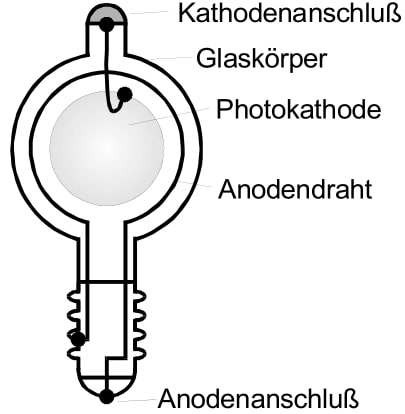
\includegraphics[width=0.5\textwidth]{images/Photozelle.jpg}
        \caption{Diese Grafik zeigt den schematischen Aufbau einer Photozelle \cite{V500}. Zusehen ist der evakuierte Glaskörper, der eine Photokathode samt Anodendraht beinhaltet.}
        \label{fig:1}
    \end{figure}
    \flushleft{Da\;}\justifying die Frequenzen des Lichts unabdingbar für die Messungen sind, muss monochromatisches, weißes Licht in dessen Spektrallinien zerlegt werden. Dies wird mithilfe des folgenden 
    Aufbaus erreicht:
    \begin{figure}[H]
        \centering
        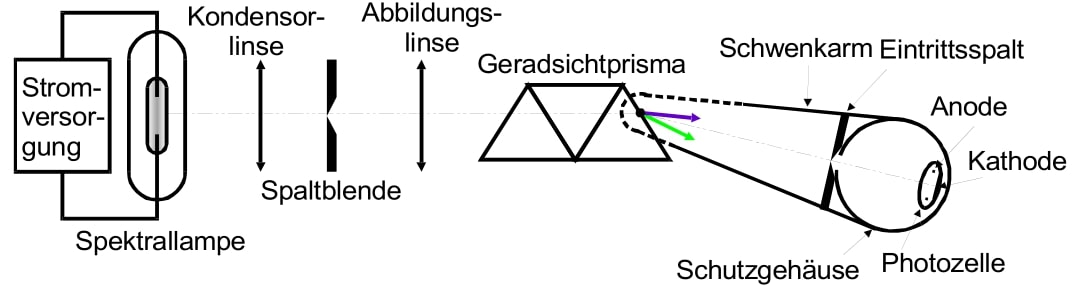
\includegraphics[width=\textwidth]{images/Schema.jpg}
        \caption{Diese Abbildung stellt den schematischen Aufbau der verwendeten Apperatur dar \cite{V500}. Auf der linke Seite befindet sich eine Spektrallampe, welche weißes, monochromatisches
        Licht erzeugt. Dieses Licht wird mithilfe der Kondesorlinse parallel auf die Spaltblende gebündelt. Das Bild des Spalts wird von der Abbildungslinse auf die Photkathode 
        abgebildet und das Geradsichtprisma zerlegt das Licht der Spektrallampe in dessen Spektrallinien.}
        \label{fig:2}
    \end{figure}
    \flushleft{Um\;}\justifying die Energie der losgelösten Elekronen zu bestimmen, wird eine variable Spannung an die Anode und Kathode der Photozelle gelegt. Dieser Strom erzeugt ein Magnetfeld, welches 
    dem Fluss der Elekronen entgegenwirkt. Diese Methode wird Gegenfeldmethode genannt und mit dem folgenden Aufbau durchgeführt:
    \begin{figure}[H]
        \centering
        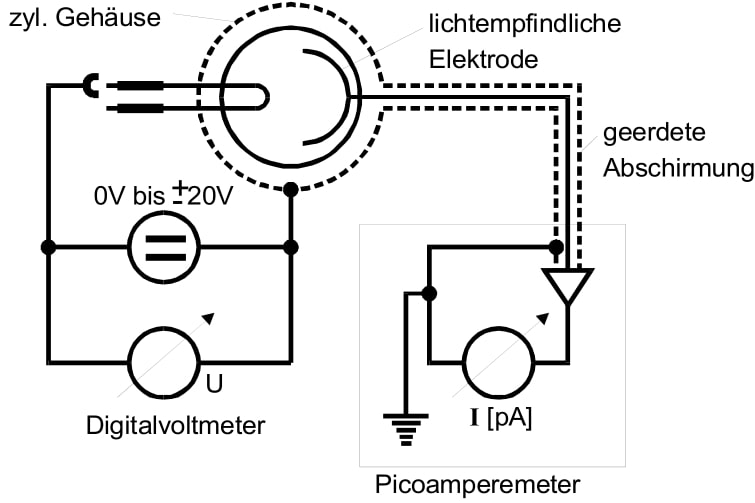
\includegraphics[width=0.75\textwidth]{images/Schaltbild.jpg}
        \caption{Diese Abbildung gibt den schematischen Aufbau der Schaltung der Photozelle wieder \cite{V500}. Mithilfe eines Digitalvoltmeters wird eine Spannung zwischen null und 
        \SI{20}{\volt} angelegt. Diese Spannung erzeugt das Gegenfeld. Das Amperemeter misst den Strom, welcher von den losgelösten Elektronen erzeugt wird.}
        \label{fig:3}
    \end{figure}
    \flushleft{Mithilfe\;}\justifying des Gegenfeldes kann die Energiebilanz aus \eqref{eq:2} erweitert werden, da die kinetische Energie der Elekronen nun gleich der elektrischen Energie $E=e_0 U_g$ sein muss, 
    wobei $e_0$ die Elementarladung und $U_g$ die variable Gegenspannung ist. Daraus ergibt sich die folgende Energiebilanz: \cite{V500}
    \begin{align}
        h\nu &= e_0 U_g + A_k \label{eq:3}
    \end{align}
    \flushleft{Durch\;}\justifying die Einführung eines Gegenfeldes wird erwartet, dass nur die Elektronen mit der größten Geschwinigkeit, also der größten kinetischen Energie, den Anodendraht erreichen. 
    Das bedeutet, dass der Photostrom bei einer bestimmten Gegenspannung augenblicklich verschwindet. Dies würde unter der Annahme auftreten, dass die Elekronen vor der Wechselwirkung
    mit dem Photon gleiche Energie besäßen. Dies ist jedoch nicht der Fall, da Elekronen einen Energieverteilung von 0 bis $\frac{1}{2}m_0 v_{\text{max}}^2$ besitzen. $m_0$ ist 
    hier die Ruhemasse eines Elekrons und $v_{\text{max}}$ die maximale Geschwinigkeit eines ausgelösten Elekrons. Folglich fällt der Photostrom nicht abrupt ab, sondern allmählich.
    Dieses Phänomen wird von der Fermi-Dirac-Statistik veranschaulicht: \cite{V500}
    \begin{figure}[H]
        \centering
        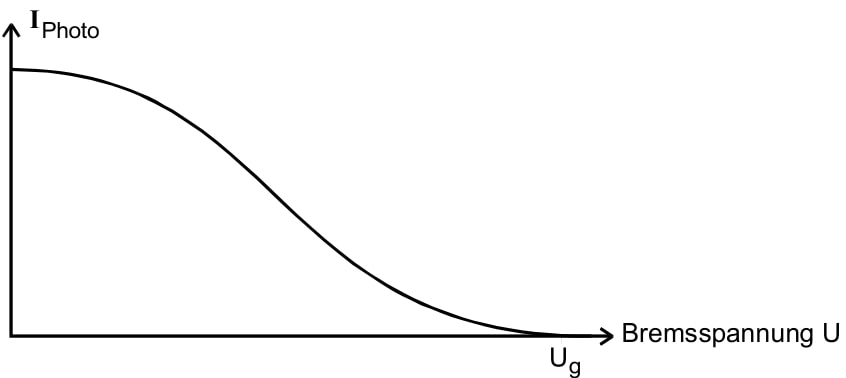
\includegraphics[width=\textwidth]{images/Dirac.jpg}
        \caption{Diese Statistik zeigt den stetigen Verlauf der Abklingkurve des Photostroms $I_{\text{Photo}}$ gegenüber der Bremsspannung $U$ \cite{V500}.}
        \label{fig:4}
    \end{figure}
    \flushleft{Da\;}\justifying nicht vorrausgesetzt werden kann, dass alle emittierten Photonen die Photokathode erreichen, ist die Fermi-Dirac-Statistik nicht aussagekräftig genug, 
    um die Gegenspannung $U_g$ zweifelsfrei zu bestimmen. Deshalb wird die parabolische Beziehung zwischen Photostrom und Bremsspannung \cite{V500}
    \begin{align}
        I_{\text{Photo}} &\propto U^2 \Leftrightarrow \sqrt{I_{\text{Photo}}} \propto U \label{eq:4}
    \end{align}
    \flushleft{verwendet,\;}\justifying um über den Schnittpunkt der entstehenden Geraden mit der x-Achse die Gegenspannung $U_g$ zu erhalten. Für die Bestimmung der Gegenspannung
    ist außerdem noch die Frequenz des einfallenden Lichts wichtig, welche sich mit der folgenden Formel bestimmen lässt:
    \begin{align}
        \nu &= \frac{c}{\lambda} \label{eq:5}
    \end{align}
    $c$ ist hier die Lichtgeschwindigkeit im Vakuum und $\lambda$ die Wellenlänge des einfallenden Lichts.

\newpage
\section{Versuchsaufbau und Durchführung}

    \flushleft{Für\;}\justifying diesen Versuch wird der folgende Aufbau verwendet:
    \begin{figure}[H]
        \centering
        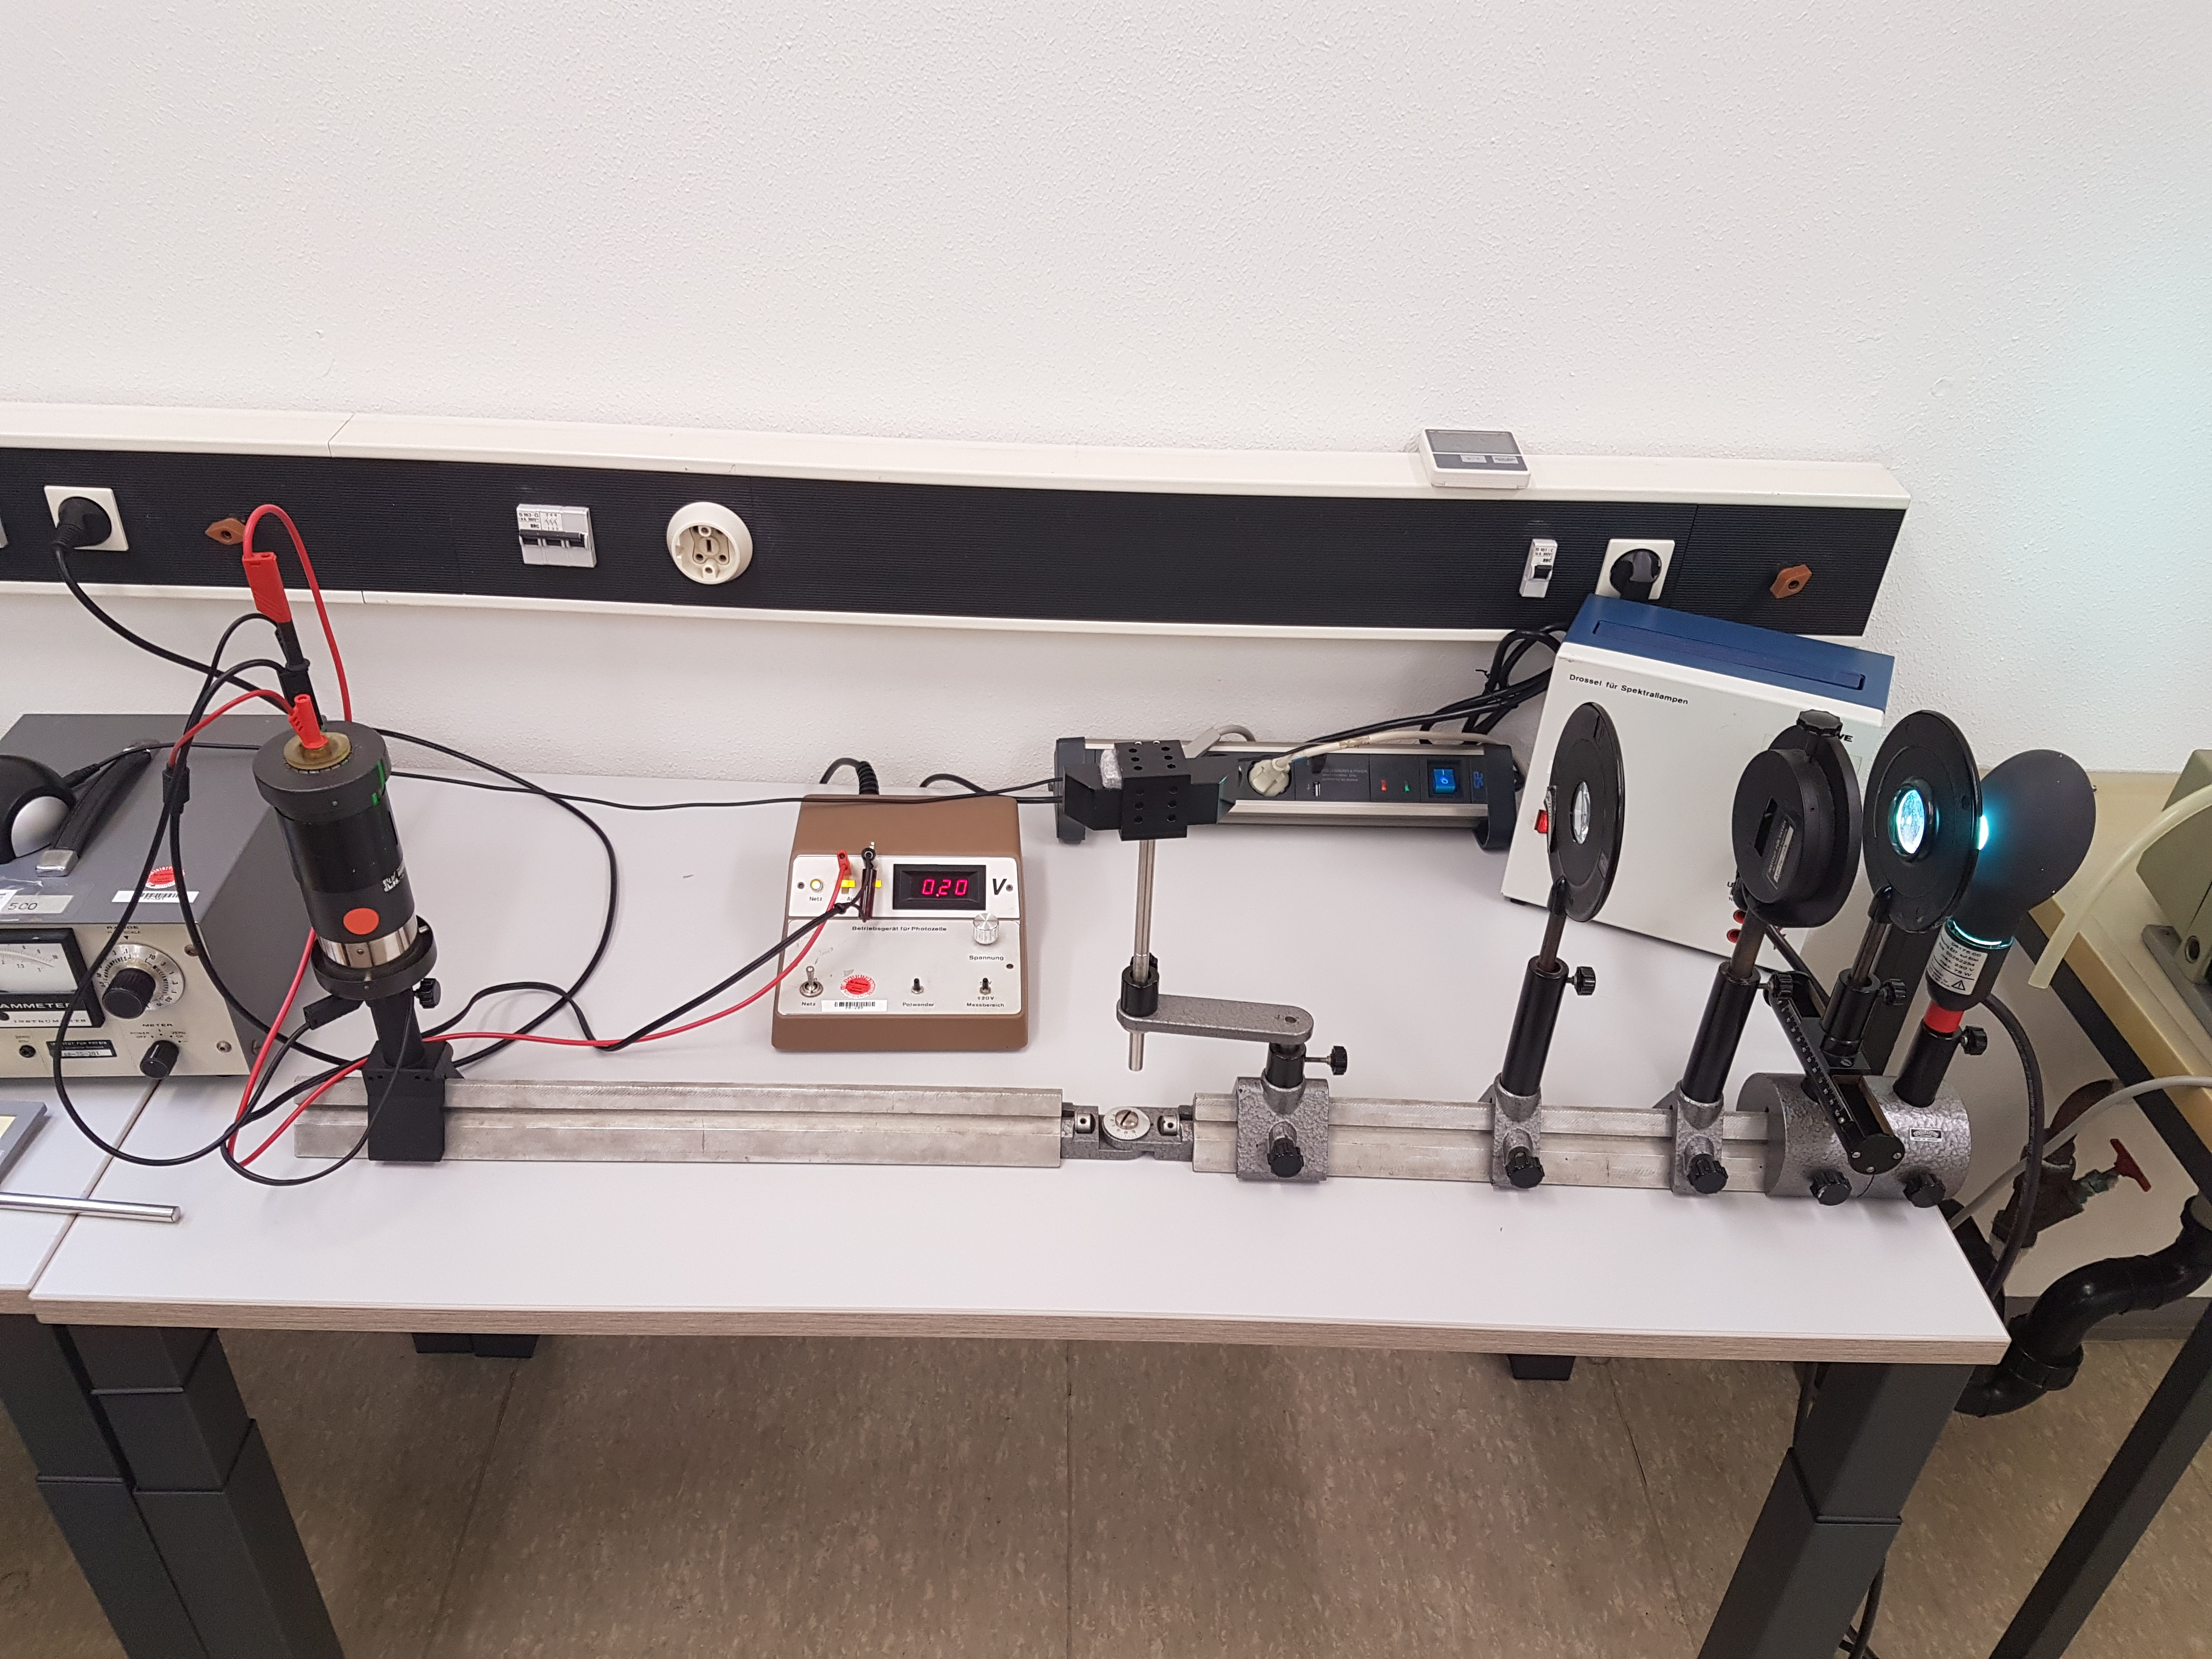
\includegraphics[width=\textwidth]{images/Aufbau.jpg}
        \caption{In dieser Abbildung ist der verwendete Versuchsaufbau zu sehen. Dieser ähnelt dem schematischen Aufbau aus Abbildung \ref{fig:2}. Hier ist die Photozelle
        auf der linken Seite. In der mitte befindet sich das Geradsichtprisma, welches über einen Schwenkarm auf der Stativschiene befestigt ist. Rechts daneben befindet 
        sich die Abbildungslinse, gefolgt von der Spaltblende. Zwischen Blende und Spektrallampe befindet sich die Kondesorlinse. An der Photozelle ist ein Digitalvoltmeter
        und ein Amperemeter angeschlossen.}
        \label{fig:5}
    \end{figure}
    \flushleft{An\;}\justifying die Photozelle werden ein Digitalvoltmeters und Amperemeter angeschlossen, mit welchen Bremsspannung und Photostrom eingestellt, beziehungsweise 
    abgelesen werden. Die hier verwendete Spektrallampe ist eine Quecksilberlampe, welche die folgenden primären Spektrallinien produziert:
    \begin{figure}[H]
        \centering
        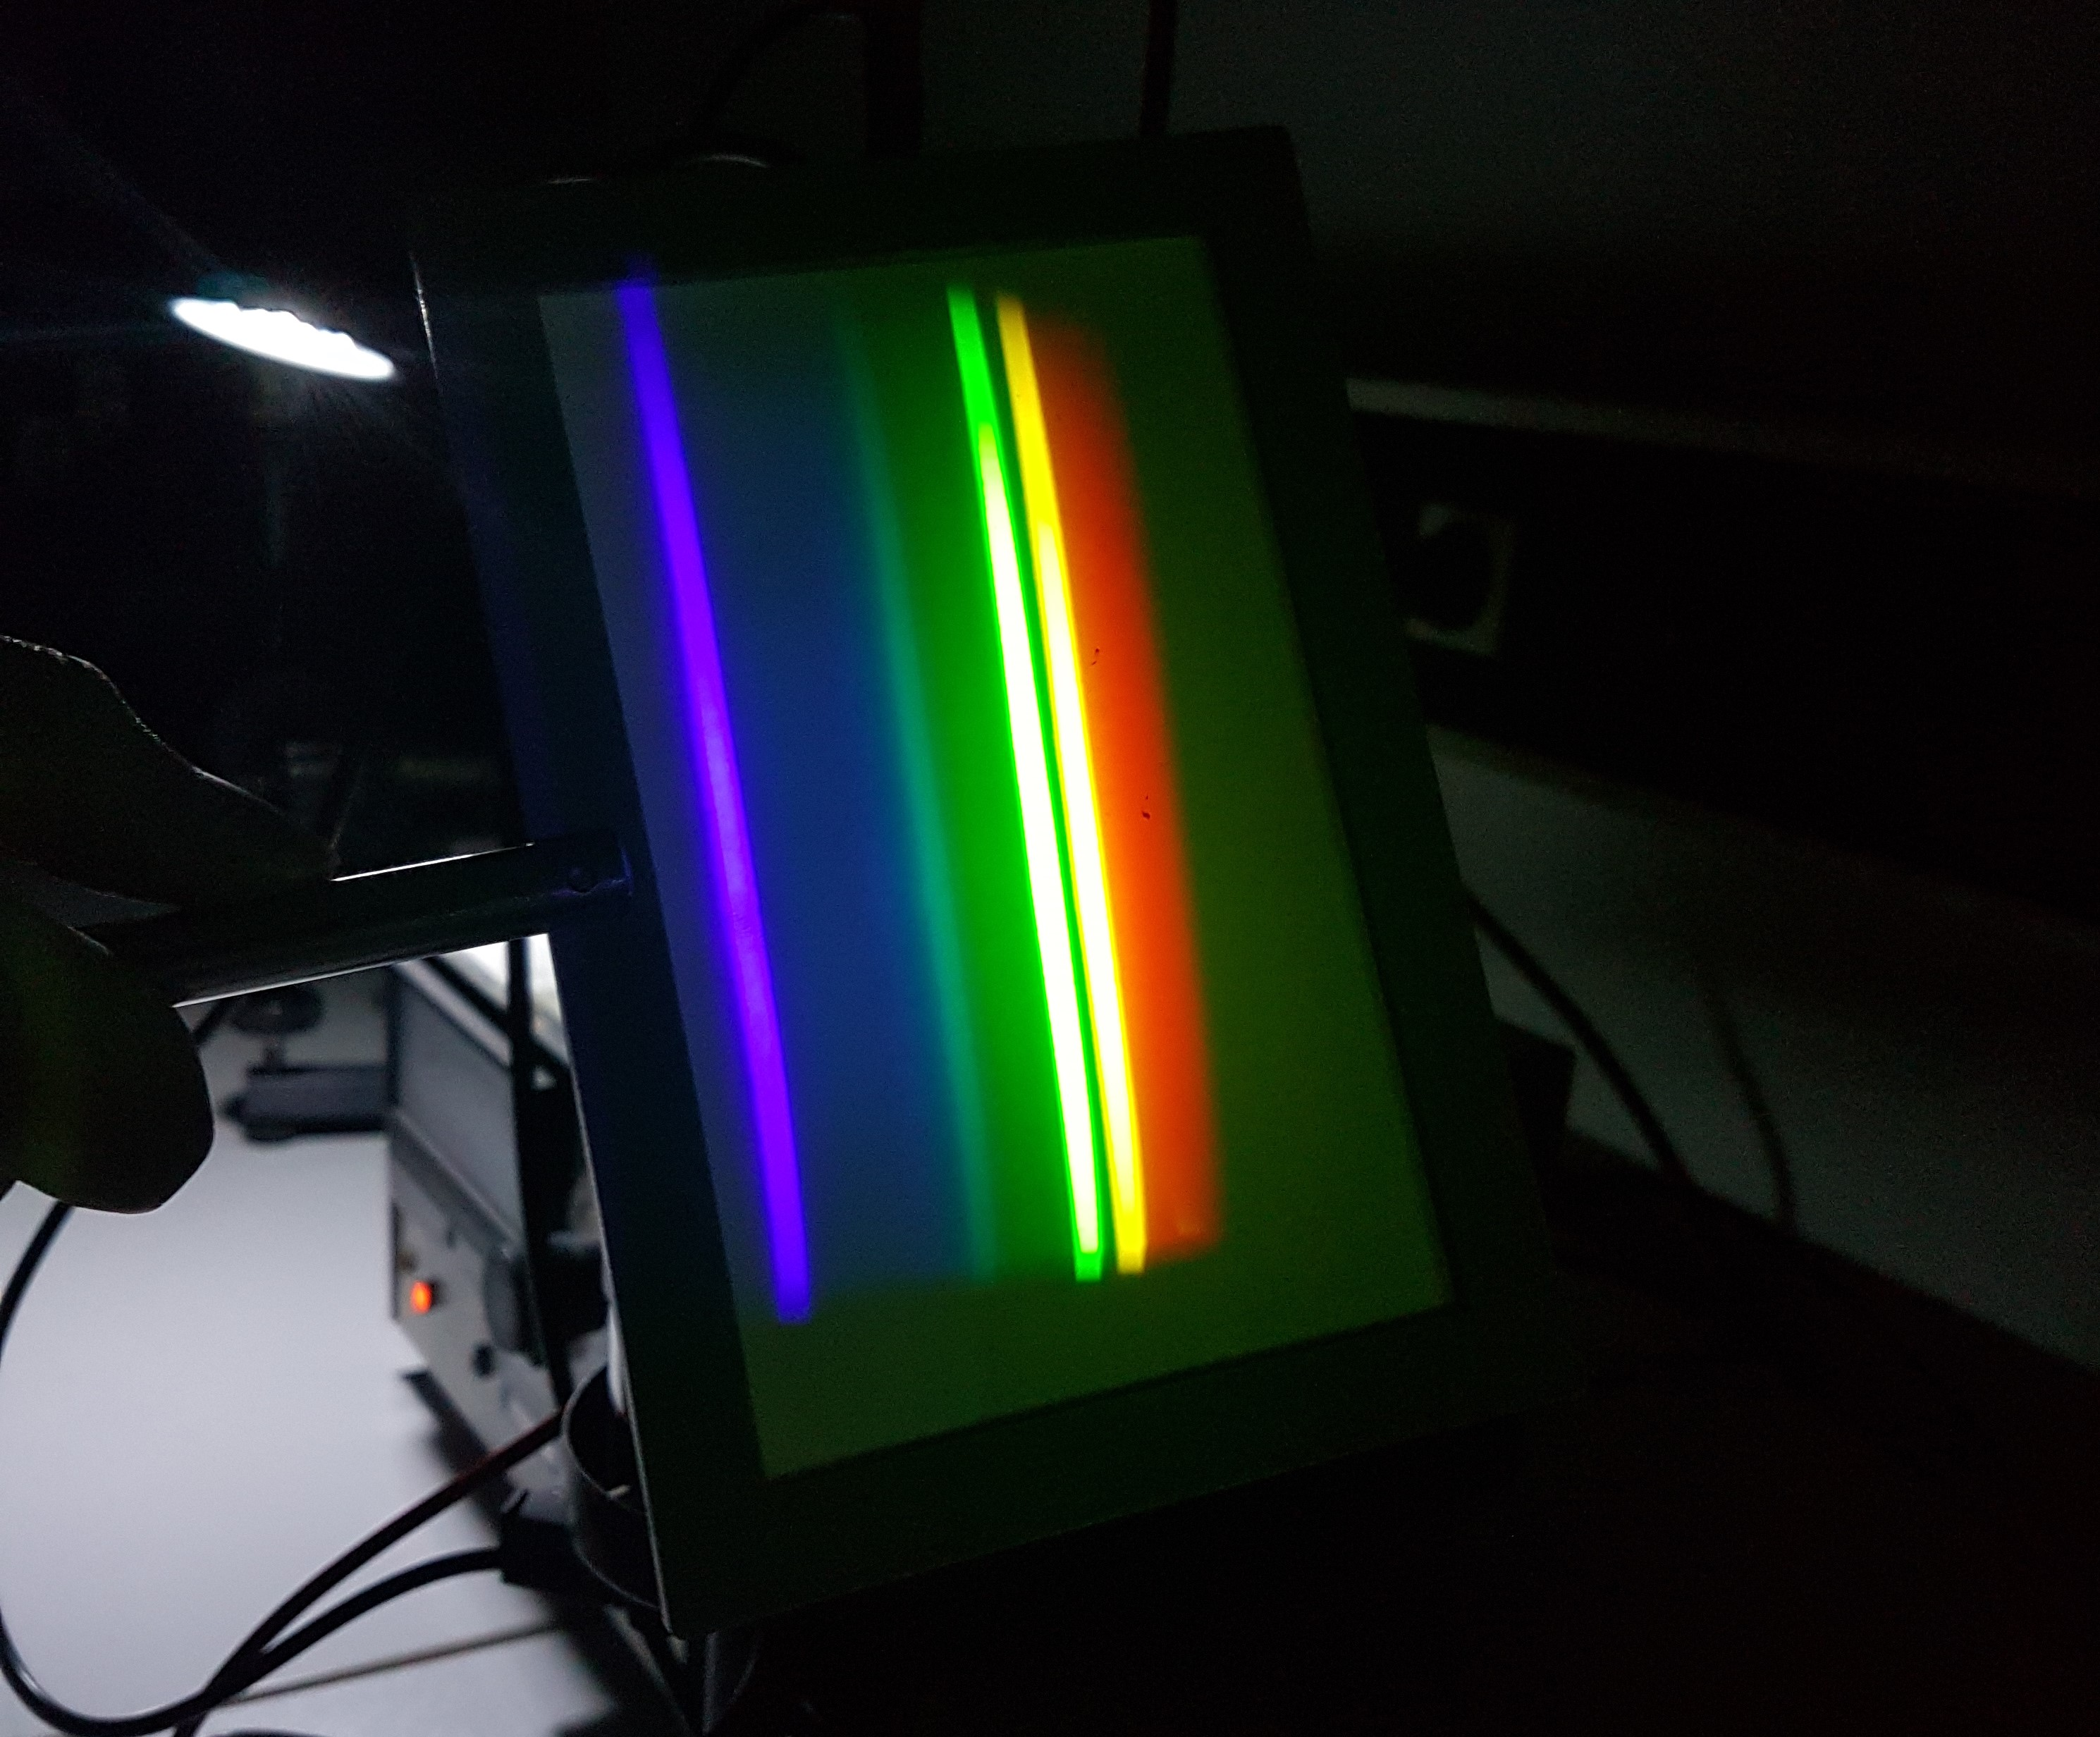
\includegraphics[width=0.5\textwidth]{images/Spektral.jpg}
        \caption{Hier ist das Spektralmuster der Quecksilberlampe zu erkennen. Deutlich zu erkennen sind die Linien violett, grün und gelb. Die in diesem Versuch gemessenen 
        Linien sind grün, gelb und rot.}
        \label{fig:6}
    \end{figure}
    \flushleft{Für\;}\justifying die gelbe Spektrallinie werden 27 Messwerte aufgenommen. Die Spannung wird in \SI{1}{\volt}-Schritten in einem Intervall von 
    \SI{18.96}{\volt} $\leq$ U $\leq$ \SI{0.02}{\volt} variiert . Dabei wird der jeweilige Photostrom dem Amperemeter entnommen. Zwischen \SI{7}{\volt} $\leq$ U $\leq$ \SI{0.5}{\volt}
    wird der Strom in \SI{0.5}{\volt}-Schritten abgelesen.
    Bei den Spektrallinien rot und grün werden je zehn Messwerte in \SI{0.2}{\volt}-Schritten aufgenommen in dem Intervall \SI{2}{\volt} $\leq$ U $\leq$ \SI{0.2}{\volt}. 

\section{Auswertung}

\subsection{Gelbe Spektrallinie}

    \flushleft{Für\;}\justifying die Auswertung werden alle Graphen mit der python Bibliothek matplotlib \cite{matplotlib} erstellt.\\
    Der folgende Graph stellt das Verhältnis zwischen der Wurzel des Photostroms $\sqrt{I_{\text{Photo}}}$ und der dazugehörigen Spannung $U$ der gelben Spektrallinie dar. Die dazu verwendeten Messwerte sind 
    in Tabelle \ref{tab:1} zu finden und es wird die Formel der allgemeinen Geradengleichung $y=mx+b$ verwendet, wobei hier $y=\sqrt{I_{\text{Photo}}}$ und $x=U$ ist. Die dazugehörigen 
    Parameter $m$ und $b$ lauten:

    \begin{align}
    m &= \text{\input{m_gelb.tex}} \label{eq:6}\\
    b &= \text{\input{b_gelb.tex}} \label{eq:7}
    \end{align}

    \begin{figure}[H]
        \centering
        \includegraphics[width=0.75\textwidth]{build/plotGelb.pdf}
        \caption{Dieser Graph stellt die Wurzel des Photostroms $\sqrt{I_{\text{Photo}}}$ der gelben Spektrallinie gegen die Bremsspannung $U$ dar. Zusehen ist ein abfallender Messverlauf, der
        bei ca. \SI{-7}{\volt} in eine lineare negative Steigung übergeht. Dieser Teil der Messreihe wurde mit einer Ausgleichsgeraden versehen, um im Anschluss die Gegenspannung
        $U_g$ durch den Schnittpunkt dieser Geraden mit der U-Achse zu bestimmen.}
        \label{fig:7}
    \end{figure}

    \flushleft{Der\;}\justifying Schnittpunkt mit der U-Achse beschreibt hier die Gegenspannung $U_g$ und wird durch Umstellen der Geradengleichung wie folgt berechnet:
    \begin{align}
    0 &= m U_g+b \Leftrightarrow -\frac{b}{m} = U_g \label{eq:8}
    \intertext{
        \flushleft{Mit\;}\justifying der Fehlerfortpflanzung der Steigung $m$
    }
    \Delta U_g &= \sqrt{ \left( -\frac{1}{m} \right)^2 \cdot \sigma_b^2 + \left( \frac{b}{2m} \right)^2 \cdot \sigma_m^2 } = \frac{1}{m} \cdot \sigma_b + \frac{b}{m^2} \cdot \sigma_m \label{eq:9}
    \intertext{
        \flushleft{und\;}\justifying dem python Befehl ufloat der uncertainties Bibliothek \cite{uncertainties} ergibt sich für die Gegenspannung:
    }
    U_g &= \text{\input{U_g_gelb_err.tex}} \label{eq:10}
    \end{align}

\newpage
\subsection{Grüne Spektrallinie}

    \flushleft{Für\;}\justifying die grüne Spektrallinie wird die Gegenspannung genauso wie bei der gelben Spektrallinie bestimmt. Der folgende Graph wird analog zur gelben 
    Spektrallinie mithilfe der Messwerte aus Tabelle \ref{tab:2} erstellt. Die dazu verwendeten Parameter $m$ und $b$ lauten wie folgt:
    \begin{align}
    m &= \text{\input{m_gruen.tex}} \label{eq:11}\\
    b &= \text{\input{b_gruen.tex}} \label{eq:12}
    \end{align}

    \begin{figure}[H]
        \centering
        \includegraphics[width=0.75\textwidth]{build/plotGruen.pdf}
        \caption{Dieser Graph gibt die Messwerte des Photostroms $\sqrt{I_{\text{Photo}}}$ der grünen Spektrallinie gegen dessen Bremsspannung $U$ wieder. Es handelt sich hier
        nur um den relativ linear abfallenden Teil der Fermi-Dirak Kurve, weshalb die Ausgleichsgerade durch alle Messwerte geht. Auch hier wird die Gegenspannung $U_g$ durch den 
        Schnittpunkt der Ausgleichsgeraden mit der U-Achse bestimmt.}
        \label{fig:8}
    \end{figure}

    \flushleft{Die\;}\justifying Gegenspannung $U_g$ wird ebenfalls analog mit Formel \eqref{eq:8} und der Fehlerfortpflanzung \eqref{eq:9} bestimmt und lautet:
    \begin{align}
    U_g &=\text{\input{U_g_gruen.tex}} \label{eq:13}
    \end{align}

\newpage
\subsection{Rote Spektrallinie}

    \flushleft{Für\;}\justifying die rote Spektrallinie wird identisch zu den anderen beiden Spektrallinien verfahren. Für den folgenden Graph werden die Messwerte aus Tabelle
    \ref{tab:3} und die Parameter
    \begin{align}
    m &= \text{\input{m_rot.tex}} \label{eq:14}\\
    b &= \text{\input{b_rot.tex}} \label{eq:15}
    \end{align}
    \flushleft{verwendet.\;}\justifying

    \begin{figure}[H]
        \centering
        \includegraphics[width=0.75\textwidth]{build/plotRot.pdf}
        \caption{Dieser Graph stellt ebenfalls nur den linear abfallenden Teil der Fermi-Dirak Kurve dar. Hier wird abermals die Gegenspannung $U_g$ durch den Schnittpunkt
        der Ausgleichsgeraden mit der U-Achse bestimmt.}
        \label{fig:9}
    \end{figure}

    \flushleft{Die\;}\justifying Gegenspannung $U_g$ der roten Spektrallinie wird wieder analog zur gelben und grünen Spektrallinie mithilfe der Formeln \eqref{eq:8} und \eqref{eq:9} 
    berechent und lautet:
    \begin{align}
    U_g &=\text{\input{U_g_rot.tex}} \label{eq:16}
    \end{align}

\newpage
\subsection{Verhältnis und Austrittsarbeit}


    \flushleft{Um\;}\justifying das Verhältnis $\sfrac{h}{e_0}$ und die Austrittsarbeit $A_K$ bestimmen zu können, werden die zuvor berechneten Gegenspannungen $U_g$
    gegen die Lichtfrequenzen der einzelnen Spektrallinien graphisch aufgetragen. Die Lichtfrequenzen werden mit der Formel
    \begin{align}
    \nu &= \frac{c}{\lambda} \label{eq:17}
    \end{align}
    \flushleft{berechnet,\;}\justifying wobei $\lambda$ die Wellenlänge und $c$ die Lichtgeschwindigkeit im Vakuum darstellt. $c$ wird der Bibliothek constants
    von scipy \cite{scipy} entnommen und die Wellenlängen der Versuchsanleitung \cite{V500}. Diese lauten:
    \begin{subequations} \label{eq:18}
    \begin{align}
    \lambda_{\text{Gelb}} &= \text{\SI{578}{\nano\meter}} \label{eq:18a}\\
    \lambda_{\text{Grün}} &= \text{\SI{546}{\nano\meter}} \label{eq:18b}\\
    \lambda_{\text{Rot}} &= \text{\SI{671}{\nano\meter}} \label{eq:18c}
    \end{align}
    \end{subequations}
    \flushleft{Werden\;}\justifying die Gegenspannungen $U_g$ gegen die folgenden Frequenzen
    \begin{subequations} \label{eq:19}
    \begin{align}
    \nu_{\text{Gelb}} &= \text{\input{f_gelb.tex}} \label{eq:19a}\\
    \nu_{\text{Grün}} &= \text{\input{f_gruen.tex}} \label{eq:19b}\\
    \nu_{\text{Rot}} &= \text{\input{f_rot.tex}} \label{eq:19c}
    \end{align}
    \end{subequations}
    \flushleft{aufgetragen,\;}\justifying unter Verwendung der umgestellten Formel \eqref{eq:3} $U_g = \frac{h}{e_0}\nu - A_K$, ergibt sich der folgende Graph:

    \begin{figure}[H]
        \centering
        \includegraphics[width=0.75\textwidth]{build/plotLambda.pdf}
        \caption{Dieser Graph trägt die zuvor bestimmten Gegenspannungen $U_g$ der Spektrallinien gelb, grün und rot gegen dessen jeweiligen Frequenzen auf. Die
        Steigung $m$ der Ausgleichsgeraden gibt das Verhältnis $\sfrac{h}{e_0}$ wieder und der Schnittpunkt der Ausgleichsgeraden mit der $U_g$-Achse die Austrittsarbeit $A_K$.}
        \label{fig:10}
    \end{figure}

    \flushleft{Die\;}\justifying dazu verwendeten Parameter $m$ und $b$ lauten
    \begin{align}
    m &= \text{\input{m_f.tex}}\;\text{und} \label{eq:20}\\
    b &= \text{\input{b_f.tex},} \label{eq:21}\\
    \end{align}
    \flushleft{wobei\;}\justifying $m$ das Verhältnis $\sfrac{h}{e_0}$ und $b$ die Austrittsarbeit $A_K$ beschreibt.

\newpage
\section{Diskussion}

     \flushleft{Die\;}\justifying Graphen der einzelnen Spektrallinie weisen einen näherungsweise linearen Abfall des Photostroms auf. Dies ist laut der Fermi-Dirac-Statistik
     zu erwarten, da die Energieverteilung der herausgelösten Elekronen nicht homogen ist. Die Gegenspannungen der gelben und grünen Spektrallinie liegen dicht beieinander,
     was aufgrund der ähnlichen Frequenzen \eqref{eq:19a} und \eqref{eq:19b} zu erwarten ist. 

    \flushleft{Das\;}\justifying Verhältnis $\sfrac{h}{e_0}$ und die Austrittsarbeit $A_K$ lauten nach dem Graphen aus Abbildung \ref{fig:10}:
    \begin{align}
        \sfrac{h}{e_0} &= \text{\input{m_f.tex}} \label{eq:22}\\
        A_K &= \text{\input{b_f.tex}} \label{eq:23}
        \intertext{
            \flushleft{Der\;}\justifying relaitve Fehler des Verhältnisses zum Literaturwert, welcher sich aus den Konstanten $h$ und $e_0$ berechnen lässt, liegt bei
        }
        Fehler_1 &= \text{\input{fehler.tex}.} \label{eq:24}
    \end{align}
    \flushleft{Das\;}\justifying planksche Wirkungsquantum $h$ und die Elementarladung $e_0$ werden der Bibliothek constants von scipy \cite{scipy} entnommen.
    Das experimentelle Verhältnis liegt sehr weit von dem erwarteten Verhältnis entfernt. Dies könnte auf den Graphen \ref{fig:9} zurückführbar sein, da die
    Gegenspannung weit im positiven Bereich liegt, obwohl rotes Licht eine geringere Energie als gelbes, oder grünes Licht besitzt. 
    Unter Betrachtung der Gegenspannung der gelben \eqref{eq:10} und der grünen Spektrallinie \eqref{eq:13}, fällt auf, dass die Gegenspannung 
    bei zunehmender Energie ebenfalls zunimmt. Also ist es unwahrscheinlich, dass die rote Spektrallinie eine stärkere Gegenspannung bei kleinerer Energie aufweist. 
    Wird demnach die Frequenz der roten Spektrallinie aus dem Graphen \ref{fig:10} entfernt und eine Gerade durch die Punkte für gelb und grün gelegt, folgt der Graph:

    \begin{figure}[H]
        \centering
        \includegraphics[width=0.75\textwidth]{build/plotLambdaL.pdf}
        \caption{Dieser Graph stellt die Gegenspannung $U_g$ der gelben und grünen Spektrallinie gegen dessen Frequenzen dar. Aus den beiden Punkten wird eine
        Gerade bestimmt. Analog zum Graphen \ref{fig:10} ist hier die Steigung der Geraden $m$ das Verhältnis $\frac{h}{e_0}$ und der Schnittpunkt der Geraden mit der
        $U_g$-Achse die Austrittsarbeit $A_K$.}
        \label{fig:10}
    \end{figure}

    \flushleft{Die\;}\justifying verwendeten Parameter $m$ und $b$ lauten wie folgt:
    \begin{align}
    m &= \frac{h}{e_0} = \text{\input{m_L.tex}} \label{eq:25}\\
    b &= A_K = \text{\input{b_L.tex}} \label{eq:26}
    \intertext{
        \flushleft{Wird\;}\justifying das neue Verhältnis mit dem Literaturwert verglichen entsteht der folgende relative Fehler:
    }
    Fehler_2 &= \text{\input{fehler_L.tex}} \label{eq:27} 
    \end{align}
    \flushleft{Der\;}\justifying neue Fehler \eqref{eq:27} ist deutlich geringer als der vorherige \eqref{eq:24}, was einen systematischen Fehler in der Messreihe der
    roten Spektrallinie vermuten lässt. Ein möglicher Grund kann die geringe Intensität des Lichtes sein, wie in Abbildung \ref{fig:6} zu erkennen ist. Eine mögliche 
    Verbesserung der Messwerte wäre, die dritte primäre Spektrallinie (violett) zu messen. Neben dem hohen relativen Fehler ist das Vorzeichen der Austrittsarbeit \eqref{eq:21}
    falsch, da ein Wert mit positiven Vorzeichen eingesetzt in die umgestellte Geradengleichung \eqref{eq:3} eine negative Austrittsarbeit bedeuten würde.

    \flushleft{Die\;}\justifying Beschleunigungsspannung erreicht einen Sättigungswert, da ab einen gewissen Punkt jedes Elekron, welches von einem Photon gestoßen wird, 
    herausgelöst wird. Das asymptotische Verhalte lässt sich damit erklären, dass nicht jedes Elekron den Weg zur Anode findet und somit nicht von Amperemeter gemessen wird. 
    Um bei einer endlichen Beschleunigungsspannung einen Sättigungswert des Photostroms erreichen zu können, sollte die Austrittsarbeit der Photokathode minimal sein und der Anodendraht
    eine größtmögliche Fläche um die Photkathode abdecken. 

    \flushleft{Der\;}\justifying Graph der gelben Spektrallinie \ref{fig:7} gibt den Verlauf des Photostroms bei sinkender Bremsspannung wieder. Wie in der Theorie bereits 
    angedeutet, würde erwartet werden, dass der Strom bei der Gegenspannung $U_g$ abrupt abfallen würde. Dies ist jedoch nicht der Fall, da sonst von einer homogenen Energieverteilung
    der Elektronen ausgegangen wird. Elekronen besitzen unterschiedliche Energien, die von $0\leq E \leq \sfrac{1}{2}m_0 v_{\text{max}}^2$ reichen kann. Demnach kommen bei steigender 
    Bremsspannung nur noch die Elekronen an der Anoode an, die am meisten Energie vor dem Stoß besitzen. Daraus ergibt sich der Kurvenverlauf der Fermi-Dirak-Statistik, welcher 
    ebenfalls im Graphen \ref{fig:7} erkennbar ist. 

    \flushleft{Da\;}\justifying das Kathodenmaterial bereits bei \SI{20}{\degree} verdampft, kann es passieren, dass sich das verdampfte Metall auf dem Anodendraht absetzt und
    seinerseits durch den Photoeffekt Elekronen emittiert. Dies kann zu einem negativen Strom führen. Da der Anodendraht eine sehr kleine Fläche im Vergleich zur Kathode besitzt, 
    ist hier die Sättigung bereits bei vergleichsweise kleinen Spannungen möglich. 

    \flushleft{Wenn\;}\justifying ein negativer Strom bei energiearmen Licht auftritt, kann eine geringe Austrittsarbeit vorrausgesetzt werden, da sich die Austrittsarbeit aus der 
    Differenz der Photonenenergie und der kinetischen Energie der Elektronen nach Formel \eqref{eq:3} zusammensetzt.

\newpage
\printbibliography

\newpage
\section{Appendix}

\begin{table}[H]
    \centering
    \caption{Diese Tabelle beinhaltet die Messwerte der Bremsspannung $U$ und der Photostromstärke $I$ der gelben Spektrallinie}
    \input{Gelb.tex}
    \label{tab:1}
\end{table}

\begin{table}[H]
    \centering
    \caption{Diese Tabelle beinhaltet die Messwerte der Bremsspannung $U$ und der Photostromstärke $I$ der grünen Spektrallinie}
    \input{Gruen.tex}
    \label{tab:2}
\end{table}

\begin{table}[H]
    \centering
    \caption{Diese Tabelle beinhaltet die Messwerte der Bremsspannung $U$ und der Photostromstärke $I$ der roten Spektrallinie}
    \input{Rot.tex}
    \label{tab:3}
\end{table}

\end{document}


